\documentclass{beamer}
\usecolortheme{rose}
\usepackage{float}
\usepackage{graphicx}
\usepackage{tikz}
\usepackage{pgfplots}
\usepackage{pgf-pie}
\usepackage{bbding}
\usepackage[utf8]{inputenc}
\usepackage{csquotes}
\usepackage[sorting=none]{biblatex}
\addbibresource{bibliography.bib}
\setbeamertemplate{bibliography item}{\insertbiblabel}
\title{Comparing WebAssembly and JavaScript for a web based photo editor}
\author{Sam Robbins}
\institute{Durham University}
\date{}



\begin{document}


\frame{\titlepage}

\begin{frame}
    \frametitle{What is the project about?}

    For a long time, JavaScript was the only method for doing computation in web browsers, however in 2017, Web Assembly was introduced as an alternative \cite{haas2017bringing}.

    \begin{definition}[Web Assembly]
        Web Assembly is a language that allows for the execution of languages that compile to assembly on the web
    \end{definition}




\end{frame}

\begin{frame}
    \frametitle{Research Question}
    Finding in which cases Web Assembly offers a benefit over JavaScript, by implementing image processing algorithms using both mechanisms.
\end{frame}

\begin{frame}
    \frametitle{Deliverables}
    \begin{itemize}
        \item \textbf{Basic aim}

              Compare the performance of one complex algorithm between Web Assembly and JPEG, for a complex algorithm, it should not simply loop over the pixels of the image, and instead be performing more sophisticated techniques.
        \item \textbf{Intermediate aim}

              Extend the basic aim to multiple complex algorithms.
        \item \textbf{Advanced aim}

              Look into tweaks that can be used to improve performance, such as compile time optimizations for Web Assembly.
    \end{itemize}
\end{frame}

\begin{frame}
    \vfill
    \centering
    \begin{beamercolorbox}[sep=8pt,center,shadow=true,rounded=true]{title}
        \usebeamerfont{title} What has been done by others?\par%
    \end{beamercolorbox}
    \vfill
\end{frame}

\begin{frame}
    \frametitle{Using Web Assembly for image processing — Next.js \cite{nextjs}}
    \begin{center}
        \includegraphics[width=5cm]{nextjs.png}

    \end{center}

    $$
        96.5 \text{ MB} \Rightarrow 69.2 \text{ MB}
    $$
\end{frame}

\begin{frame}
    \frametitle{Performance of Web Assembly — Figma \cite{figmawasm}}
    \begin{center}
        \includegraphics[width=10cm]{figma_perf.png}

    \end{center}

    \begin{center}
        3$\times$ faster load times
    \end{center}
\end{frame}

\begin{frame}
    \frametitle{Performance of Web Assembly — Fastq.bio \cite{fastq}}
    \begin{center}
        \includegraphics[width=10cm]{fastq.png}

    \end{center}
\end{frame}

\begin{frame}
    \frametitle{Performance of Web Assembly — Compared to native \cite{jangda2019not}}

    {\small
        \begin{table}[H]
            \centering
            \vspace*{6pt}
            \label{native}
            \begin{tabular}{cccc}\hline\hline
                Benchmark & Field                   & Native time(s) & Google Chrome time(s) \\ \hline
                bzip2     & Compression             & 370            & 864                   \\
                mcf       & Combinatorial           & 221            & 180                   \\
                milc      & Chromodynamics          & 375            & 369                   \\
                namd      & Molecular Dynamics      & 271            & 369                   \\
                gobmk     & Artificial Intelligence & 352            & 537
            \end{tabular}
        \end{table}
    }
\end{frame}

\begin{frame}
    \frametitle{How does it compare?}
    \begin{itemize}
        \item Studies haven't been done on the performance of web assembly for image processing, just some metrics found during development of one project
        \item Often comparisons are being made between asm.js and Web Assembly, comparing native implementations gives a more fair comparison
    \end{itemize}
\end{frame}

\begin{frame}
    \vfill
    \centering
    \begin{beamercolorbox}[sep=8pt,center,shadow=true,rounded=true]{title}
        \usebeamerfont{title} My Solution\par%
    \end{beamercolorbox}
    \vfill
\end{frame}

\begin{frame}
    \frametitle{Choosing a language for Web Assembly}
    \begin{itemize}
        \item Most languages have some support for Web Assembly
        \item Web Assembly doesn't include a garbage collector so languages that don't need them are preferred
        \item Lots of development work has been put into the Rust ecosystem regarding web assembly
    \end{itemize}


\end{frame}

\begin{frame}
    \frametitle{Choosing problems}
    \begin{itemize}
        \item Common image processing tasks
        \item Range of computational complexity
    \end{itemize}
\end{frame}

\begin{frame}
    \frametitle{Platform}
    \begin{itemize}
        \item Want results to be equivalent to Google Chrome (64\% market share \cite{webmarketshare})
        \item Node.js uses the V8 browser engine (the same as Google Chrome)
    \end{itemize}
\end{frame}

\begin{frame}
    \frametitle{Brightness}
    \begin{center}
        \includegraphics[width=0.48\textwidth]{default.png}
        \includegraphics[width=0.48\textwidth]{bright.png}
    \end{center}

\end{frame}

\begin{frame}
    \frametitle{Contrast}
    \begin{center}
        \includegraphics[width=0.48\textwidth]{default.png}
        \includegraphics[width=0.48\textwidth]{contrast.png}
    \end{center}

\end{frame}

\begin{frame}
    \frametitle{Gaussian Blur}
    \begin{center}
        \includegraphics[width=0.48\textwidth]{default.png}
        \includegraphics[width=0.48\textwidth]{blur.png}
    \end{center}

\end{frame}

\begin{frame}
    \frametitle{JPEG — YCbCr Conversion \cite{jpeg}}
    \begin{center}
        \includegraphics[width=0.48\textwidth]{ycbcr.png}
    \end{center}
\end{frame}

\begin{frame}
    \frametitle{JPEG — Downsampling}
    \begin{center}
        \includegraphics[width=0.8\textwidth]{downsampling.png}
    \end{center}
\end{frame}

\begin{frame}
    \frametitle{JPEG — DCT \cite{ken1998image}}
    $$
        T_{i,j}=\begin{cases}
            1/\sqrt{N}                                    & \text{if } i=0 \\
            \sqrt{\frac{2}{N}}\cos(\frac{(2j+1)i\pi}{2N}) & \text{if } i>0 \\
        \end{cases}
    $$

    N is the dimension of the matrix (here 8)
\end{frame}

\begin{frame}
    \frametitle{JPEG — Quantization}
    $$
        \begin{bmatrix}
            16 & 11 & 10 & 16 & 24  & 40  & 51  & 61  \\
            12 & 12 & 14 & 19 & 26  & 58  & 60  & 55  \\
            14 & 13 & 16 & 24 & 40  & 57  & 69  & 56  \\
            14 & 17 & 22 & 29 & 51  & 87  & 80  & 62  \\
            18 & 22 & 37 & 56 & 68  & 109 & 103 & 77  \\
            24 & 35 & 55 & 64 & 81  & 104 & 113 & 92  \\
            49 & 64 & 78 & 87 & 103 & 121 & 120 & 101 \\
            72 & 92 & 95 & 98 & 112 & 100 & 103 & 99
        \end{bmatrix}
    $$
\end{frame}

\begin{frame}
    \frametitle{JPEG — Zigzag}
    \begin{center}
        \includegraphics[width=0.7\textwidth]{zigzag.png}
    \end{center}
\end{frame}

\begin{frame}
    \frametitle{Web Assembly Optimizations}
    \begin{enumerate}
        \item Link Time Optimization


        \item Rust compiler opt-level

              \begin{itemize}
                  \item "s" : optimize for size
                  \item "z" : optimize aggressively for size
              \end{itemize}


        \item \texttt{wasm-opt}



              \begin{itemize}
                  \item \texttt{-Os} : optimize for size
                  \item \texttt{-Oz} : optimize aggressively for size
                  \item \texttt{-O} : optimize for speed
                  \item \texttt{-O3} : optimize aggressively for speed
              \end{itemize}

    \end{enumerate}
\end{frame}

\begin{frame}
    \frametitle{Web Assembly Optimizations - Time}
    \begin{figure}[H]
        \centering
        \begin{tikzpicture}
            \begin{axis}[
                    symbolic x coords={No changes, LTO, Opt-s, Opt-z, -Os, -Oz, -O, -O3},
                    xtick=data,
                    x tick label style={rotate=45, anchor=north east, inner sep=0mm},
                    bar width = 20,
                    enlarge x limits = 0.1,
                    ybar,
                    ylabel = Time(Milliseconds),
                    y label style={at={(axis description cs:-0.01,.5)},anchor=south},
                    ymin=0,
                    nodes near coords,
                    axis x line*=bottom,
                    axis y line*=left,
                    width=300,
                    height=200		]
                \addplot coordinates {
                        (No changes,  1031)
                        (LTO, 846)
                        (Opt-s, 2275)
                        (Opt-z, 3846)
                        (-Os, 1078)
                        (-Oz, 1087)
                        (-O, 1154)
                        (-O3, 1028)
                    };
            \end{axis}
        \end{tikzpicture}
    \end{figure}

\end{frame}

\begin{frame}
    \frametitle{Web Assembly Optimizations - Size}
    \begin{figure}[H]
        \centering
        \begin{tikzpicture}
            \begin{axis}[
                    symbolic x coords={No changes, LTO, Opt-s, Opt-z, -Os, -Oz, -O, -O3},
                    xtick=data,
                    x tick label style={rotate=45, anchor=north east, inner sep=0mm},
                    bar width = 20,
                    enlarge x limits = 0.1,
                    ybar,
                    ylabel = Size(Kilobytes),
                    y label style={at={(axis description cs:-0.01,.5)},anchor=south},
                    ymin=0,
                    nodes near coords,
                    axis x line*=bottom,
                    axis y line*=left,
                    width=300,
                    height=200		]
                \addplot coordinates {
                        (No changes,  1100)
                        (LTO, 920.7)
                        (Opt-s, 954.2)
                        (Opt-z, 979.5)
                        (-Os, 981.5)
                        (-Oz, 981.4)
                        (-O, 981.5)
                        (-O3, 984.2)
                    };
            \end{axis}
        \end{tikzpicture}
    \end{figure}
\end{frame}

\begin{frame}
    \frametitle{Verifying the results}
    \begin{figure}[H]
        \centering
        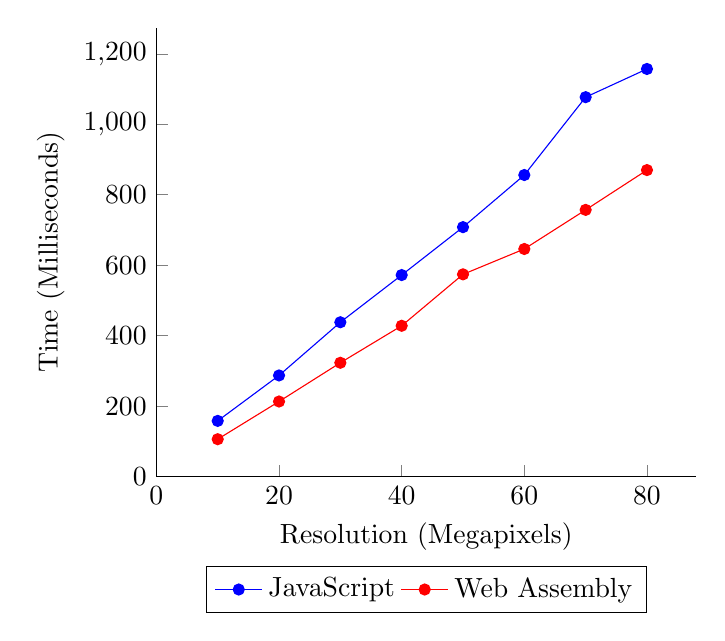
\begin{tikzpicture}
            \begin{axis}[
                    xlabel={Resolution (Megapixels)},
                    ylabel={Time (Milliseconds)},
                    xmin=0,
                    ymin=0,
                    axis x line*=bottom,
                    axis y line*=left,
                    legend style={at={(0.5,-0.2)},
                            anchor=north,legend columns=-1}
                ]

                \addplot[
                    color = blue,
                    mark=*,
                ]
                coordinates {
                        (10, 158)(20,287)(30,438)(40,572)(50,708)(60,856)(70,1077)(80,1157)
                    };
                \addplot[mark=*, color=red] coordinates {
                        (10, 106)(20,213)(30,323)(40,428)(50,574)(60,646)(70,757)(80,870)
                    };
                \legend{JavaScript, Web Assembly}

            \end{axis}
        \end{tikzpicture}

    \end{figure}
\end{frame}

\begin{frame}
    \vfill
    \centering
    \begin{beamercolorbox}[sep=8pt,center,shadow=true,rounded=true]{title}
        \usebeamerfont{title} Results\par%
    \end{beamercolorbox}
    \vfill
\end{frame}

\begin{frame}
    \frametitle{Interesting metrics}
    \begin{itemize}
        \item Run time
        \item Memory consumption
    \end{itemize}
\end{frame}

\begin{frame}
    \frametitle{Complex Algorithms}
    \begin{figure}[H]
        \centering
        \begin{tikzpicture}
            \begin{axis}[
                    symbolic x coords={JavaScript, Web Assembly},
                    xtick=data,
                    bar width = 20,
                    enlarge x limits = 0.5,
                    ybar,
                    ylabel = Time(Seconds),
                    ymin=0,
                    nodes near coords,
                    axis x line*=bottom,
                    axis y line*=left,
                    width=200,
                    legend style={at={(0.5,-0.15)},
                            anchor=north,legend columns=-1}		]
                \addplot coordinates {
                        (JavaScript,   2.48)
                        (Web Assembly,  1.60)
                    };
                \addplot coordinates {
                        (JavaScript,   12)
                        (Web Assembly,  1.14)
                    };
                \legend{JPEG Encoding,Gaussian Blur}
            \end{axis}
        \end{tikzpicture}
    \end{figure}
\end{frame}

\begin{frame}
    \frametitle{Simple Algorithms}

    \begin{figure}[H]
        \centering
        \begin{tikzpicture}
            \begin{axis}[
                    symbolic x coords={JavaScript, Web Assembly},
                    xtick=data,
                    bar width = 20,
                    enlarge x limits = 0.5,
                    ybar,
                    ylabel = Time(Milliseconds),
                    ymin=0,
                    nodes near coords,
                    axis x line*=bottom,
                    axis y line*=left,
                    width=200,
                    legend style={at={(0.5,-0.15)},
                            anchor=north,legend columns=-1}		]
                \addplot coordinates {
                        (JavaScript,   102)
                        (Web Assembly,  77)
                    };
                \addplot coordinates {
                        (JavaScript,   103)
                        (Web Assembly,  278)
                    };
                \legend{Brightness, Contrast}
            \end{axis}
        \end{tikzpicture}
    \end{figure}

\end{frame}

\begin{frame}
    \frametitle{Time for the full process}
    \begin{figure}[H]
        \centering
        \begin{tikzpicture}
            \begin{axis}[
                    symbolic x coords={JavaScript, Web Assembly, imagemagick},
                    xtick=data,
                    bar width = 20,
                    enlarge x limits = 0.2,
                    ybar,
                    ylabel = Time(Seconds),
                    ymin=0,
                    nodes near coords,
                    axis x line*=bottom,
                    axis y line*=left,
                    width=300,
                    height=200		]
                \addplot coordinates {
                        (JavaScript,  3.17)
                        (Web Assembly,  2.79)
                        (imagemagick,  0.37)
                    };
            \end{axis}
        \end{tikzpicture}
    \end{figure}
\end{frame}

\begin{frame}
    \frametitle{Memory consumption of the full process}
    \begin{figure}[H]
        \centering
        \begin{tikzpicture}
            \begin{axis}[
                    symbolic x coords={JavaScript, Web Assembly, imagemagick},
                    xtick=data,
                    bar width = 20,
                    enlarge x limits = 0.2,
                    ybar,
                    ylabel = Memory (Megabytes),
                    ymin=0,
                    nodes near coords,
                    axis x line*=bottom,
                    axis y line*=left,
                    width=300,
                    height=200		]
                \addplot coordinates {
                        (JavaScript,  61.4)
                        (Web Assembly,  28.8)
                        (imagemagick,  10.6)
                    };
            \end{axis}
        \end{tikzpicture}
    \end{figure}
\end{frame}




\begin{frame}
    \frametitle{Evaluation}
    \begin{itemize}
        \item[\Checkmark] Faster
        \item[\Checkmark] Lower memory consumption
        \item[\Checkmark] Static types
        \item[\XSolidBrush] Static types
        \item[\XSolidBrush] Slower than native
        \item[\XSolidBrush] Need to use multiple languages
        \item[\XSolidBrush] Libraries have had less development
    \end{itemize}
\end{frame}

\begin{frame}
    \frametitle{Further Work}
    \begin{itemize}
        \item WebGPU \cite{webgpu}
        \item Different methods
        \item Different languages
    \end{itemize}
\end{frame}

\begin{frame}[allowframebreaks]
    \frametitle{References}
    \printbibliography
\end{frame}

\end{document}